\documentclass{article}
\usepackage{tkz-tab}
\usepackage{amsmath} 
\usepackage{geometry}
\usepackage{indentfirst}
\setlength{\parindent}{0cm} % Retrait du paragraphe
\geometry{
    left=1cm }
\begin{document}
\underline{Tableau de variation de $f(x)$}\\
                   
$f(x)=\left(x - 2\right) \left(x - 1\right) \left(x + 1\right) \left(x + 2\right)$\\
$f'(x)=\left(x - 2\right) \left(x - 1\right) \left(x + 1\right) + \left(x - 2\right) \left(x - 1\right) \left(x + 2\right) + \left(x - 2\right) \left(x + 1\right) \left(x + 2\right) + \left(x - 1\right) \left(x + 1\right) \left(x + 2\right)$\\

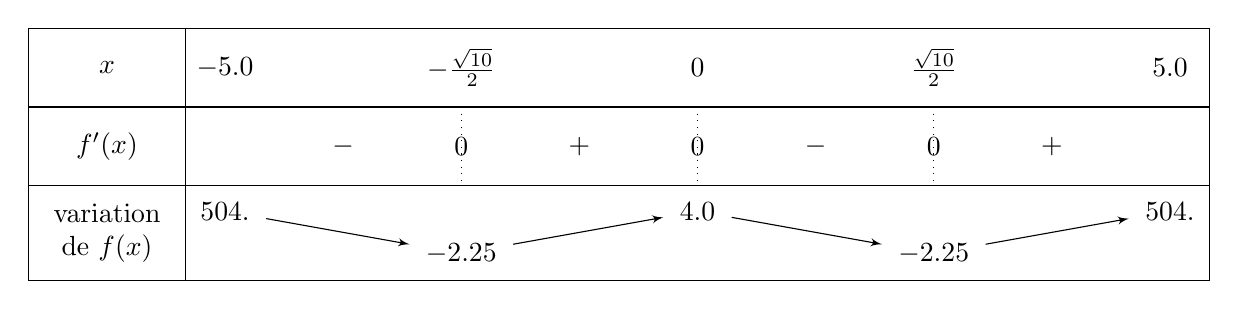
\begin{tikzpicture}
\tkzTabInit[espcl=3]{$x$ / 1 , $f'(x)$ / 1, variation de $f(x)$/1.2}
{$-5.0$,$- \frac{\sqrt{10}}{2}$,$0$,$\frac{\sqrt{10}}{2}$,$5.0$}
\tkzTabLine{,-,z,+,z,-,z,+}
\tkzTabVar{+/$504.$,-/$-2.25$,+/$4.0$,-/$-2.25$,+/$504.$}
\end{tikzpicture}
\end{document}